\chapter{Introduction}\label{chp:introduction}

\todo{Write stuff as introduction. Or not. Is it needed?}

The goal of this project is to maximize user utility in video conference solutions. To maximize utility, we need to have a well-defined sense of what that implies.

\section{Previous Work}

\cite{bruun} developed the initial Talk+ application for Comoyo, making them set on becoming an online telephone available to anyone, anywhere.

\section{Context and utility}

When defining user utility, context is everything. You have different expectations to audiovisual quality on a desktop computer with fiber connectivity compared to your phone on 3G. But how can this difference be quantized? Certainly it's not a question of screen resolution, as most smart phones today have the same 1080p resolution as most computer screens. Resolutions beyond 1080p like we can find on some "retina" screens are not that interesting for video conferencing, as the webcam producing the source video is unlikely to be able to match that.

However, physical screen size matters. Viewing distance matters. Latency matters very much. Bandwidth matters. Packet loss matters. Most of these should be fairly easy to estimate, but then we have a new problem: which of these attributes do we prioritize? Finding the optimal balance is the key to optimizing user utility. There are of course also non-technical factors that affects the expected experience quite much that cannot be determined by the device itself. For example, even though the device is the same, you'll have different expectations sitting on the bus to work compared to sitting in a sofa in your living room, even though the device is the same. Environment matters. Mood matters. Time of day probably matters. We will however not take all of these factors into account, but limit our scope to the device itself, and since the intended application is to WebRTC, what we can relatively easy determine through the browser.

There will also be diminishing returns on most of these metrics. If you have practically unlimited bandwidth available, there's little to gain from sending video with bitrates in excess of 3 Mbps, you'll just be wasting bandwidth, CPU and battery. If we define a quality threshold for a device as the "optimal" experience that can be attained as 1.0, there's no reason to try to push this as high as possible. We can though assume that all metrics that are lower than what's necessary for this optimal experience will subtract from this quality metric somehow. For example, if we say that the threshold for optimal latency for a device is \(20ms\), we can imagine a \gls{utility function} that behaves like \(arctan(c-x)\), like illustrated in \autoref{fig:utility-latency}.

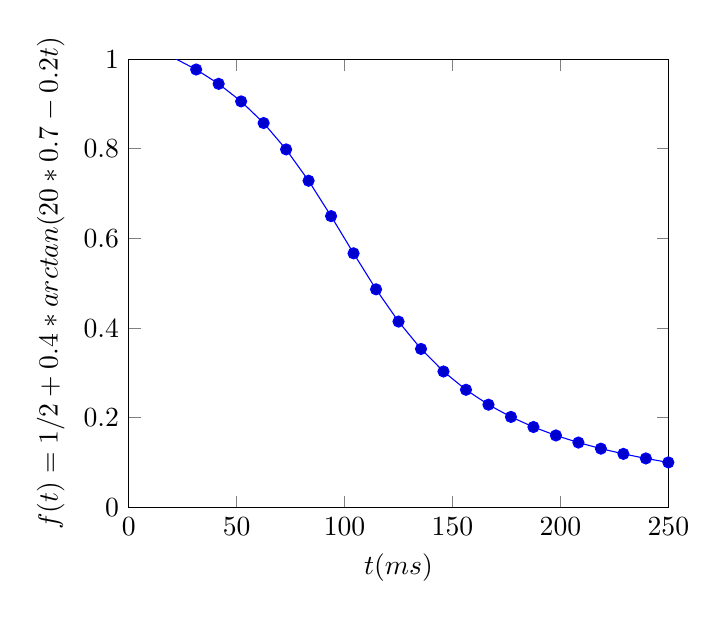
\begin{tikzpicture}
    \begin{axis}[
        xlabel={$t (ms)$},
        ylabel={$f(t) = 1/2 + 0.4*arctan(20*0.7-0.2t)$},
        xmin=0,
        ymin=0,
        ymax=1,
        xmax=250]

    \addplot+[domain=0:250]{0.6 + 0.4*rad(atan(20*0.1 - 0.02*x))};
    \label{fig:utility-latency}
    \end{axis}
\end{tikzpicture}

For now we'll assume that we have a function similar to the one illustrated in \autoref{fig:utility-latency}, returning a value approximately in the range \(1 -- 0\), for each of the metrics that comprise the user utility. Multiplying these together we'll get a user utility that lies in the same range.

Assuming this user utility function, we have to figure out what to optimize in a conversation. If a single party in a conversation experiences high latencies and much packet loss, it's likely to negatively affect the experience of all the other parties as well. We'll thus focus on maximizing the minimum utility experienced in a conversation, and then gradually improve the utility for all users ordered by their current utility in ascending order.

But before we start trying to find a optimal solution to the problem, let's see what's the status quo. To do this, we define a couple of example conversation configurations, as given in \autoref{tab:example-conversations}.

\todo{Maybe graph these on a map to illustrate the latencies between them and the servers?}
\begin{center}
    \label{tab:example-conversations}
    \begin{tabular}{| l | l |}
    \hline
    \textbf{Case} & \textbf{Devices} \\ \hline
    Chat & A (laptop, 20/5), B (laptop, 30/15) \\ \hline
    Casual & A (laptop, 10/2), B (laptop, 30/5), C(phone, 2/1) \\ \hline
    Business & A (desktop, 50/50), B (desktop) \\ \hline
    \end{tabular}
\end{center}

Are there any trivial cases we can ignore? As long as there's only two people in a conversation, and they have fairly low latency between each other and sufficient bandwidth, peer-to-peer is the optimal choice in all cases. Initially, it might seem like this would indeed be the case in all conversations with two participants, and not just the good bandwidth, small latency case. However, this is not the case. To illustrate why, consider a conversation between two people, one in Europe and one in Asia. The latency between them is ~350ms. They both have fairly acceptable bandwidths, with 3Mbps each, which should be plenty to sustain an acceptable video link between them. This, however, is not the case, as the bandwidth between them is far more limited due to the long distance and many hops through publicly routed networks. However, each of the peers has a datacenter of a distributed VPS provider nearby, to which they can utilize their full bandwidth. And these distributed VPS providers tend to have established high-quality routes between their own datacenters, SLA-backed and with all the bells and whistles you don't get on your private Internet connection. Thus, the available bandwidth between the two datacenters is far greater than what can be achieved directly between the two peers. Thus, their video link can be improved by routing their traffic through the datacenters, thus enabling each peer to utilize the full bandwidth of their connection.\footnote{This is backed by a simple experiment, using DigitalOcean as our VPS provider. From a 100Mbit university connection in Norway, sustained datarates to their Singapore datacenter varied greatly, measuring 90kBps, 3,7MBps, 1,9MBps and 2,58MBps for each test. However, from their Amsterdam datacenter, a consitent throughput of 24,6MBps was measured} Do however note that the latency is close to unchanged from routing through the datacenters, only sustained bandwidth between the peers is improved.

These conversations are not extensive, but should cover enough corner cases to be able to highlight the pros and cons of the different topologies. The examples cover the low-latency, few peers conversations; the bandwidth-challenged cases; the high-latency conversations; and the very hetrogenous device conversations, where one or more party is severly challenged in terms of either bandwidth or latency.

We assume that the backend networks are not saturated, and that each user is bandwidth-constrained only by their connection. By extension, the maximum bandwidth attainable between any pair of nodes in our network is the lesser of the upload bandwidth of the sending party and the download bandwidth of the receiving party. However, latency has to be defined for any pair of the nodes in the network, as this is mostly determined by their geographical location in relation to each other. To best illustrate the physical topology, we can draw each scenario as a complete graph:

\begin{figure}[ht!]
\centering
    \digraph{exampleconvchat}{
        edge [dir=none];
        rankdir=LR;
        a [label="A (20/5)"];
        b [label="B (30/15)"];

        a -> b [label="8ms"];
    }
    \caption{Example conversation "chat".}\label{fig:example-conv-chat}
\end{figure}

\begin{figure}[ht!]
\centering
    \digraph{exampleconvcasual}{
        edge [dir=none];
        rankdir=LR;
        a [label="A (10/2)"];
        b [label="B (30/5)"];
        c [label="C (2/1)"];

        a -> b [label="5ms"];
        a -> c [label="10ms"];
        b -> c [label="15ms"];
    }
    \caption{Example conversation ``casual''}\label{fig:example-conv-casual}
\end{figure}

\begin{figure}[ht!]
\centering
    \digraph{exampleconvbusiness}{
        edge [dir=none];
        a [label="A (50/50)"];
        b [label="B (50/50)"];
        c [label="C (50/50)"];
        d [label="D (30/30)"];
        e [label="E (30/30)"];

        a -> b [label="2ms"];
        a -> c [label="2ms"];
        a -> d [label="150ms"];
        a -> e [label="150ms"];
        b -> c [label="2ms"];
        b -> d [label="150ms"];
        b -> e [label="150ms"];
        c -> d [label="150ms"];
        c -> e [label="150ms"];
        d -> e [label="2ms"];

        {rank=same; a; c;}
        {rank=same; d; e;}
    }
    \caption{Example conversation ``business''}\label{fig:example-conv-business}
\end{figure}


\section{CPU limitations}

The naïve approach to encoding the videostreams is to encode the raw stream from the web camera into several client-optimized streams for transmission. Using VP8, this is the only way to do it. However, H.264 can be encoded in a \gls{svc} manner, which makes it possible to extract different bandwidth-streams from a single stream. With VP8 this is sadly not possible, and the only alternative is to utilize \gls{simulcast}, a technique that sends several streams to the same endpoint, which can then select which of the streams to forward to the different endpoints. This is not as efficient as sending only a single stream however, and the encoding step is also costlier on the CPU.

\todo{Write about the future of H.264/VP9, SVC, hardware acceleration, etc}


\section{Approaching a solution}

We've now seen the problem domain, we've seen some of the current approaches to the problem and how they perform, and we have an inkling of thought that says that the there's lots of room for improvement. From the graphs we've drawn up of the example conversations, it's clear that we can find better topologies than what's currently available. My suggestion is to use the utility function we described earlier to calculate the utility gained from a given topology, and then use a modified shortest-path algorithm from each client to find the optimal routing to all the other clients.

Should the solution be computed locally at each client how to route it's data, or centrally by the room?

    Client:
        - Easy to maximize returns
        - Doesn't prioritize any traffic for others
        - Allows the client to specify encoding servers and their relative cost
        - Client knows best his own capabilities and resources
        - Still requires consent from partner on bw usage and quality

    Room:
        - Centralized logic
        - Knows the full state of the room
        - Can take all parties into account

Can it be modelled as a game, and an approach estimated from game theory?

\section{Terminology}

When we talk about topology in this thesis, a topology is intended as one given configuration of who sends data where. It's thus unrelated to devices or hardware network topologies. \todo{Better word needed?} This is thus purely a logical term, as the physical topology will be assumed constant for our experiements. However, it's in the logic the magic happens.
